\documentclass[article,shortnames]{jss}

%% -- LaTeX packages and custom commands ---------------------------------------

%% recommended packages
\usepackage{thumbpdf,lmodern}

%% further packages
\usepackage{amsmath,amssymb}
\usepackage{dsfont}
\usepackage[figuresright]{rotating}
\usepackage{array}
\usepackage{orcidlink}

%% custom commands (from preamble.tex of the R Journal version)
\newcommand{\R}{\mathds{R}}
\newcommand{\yes}{\checkmark}
\newcommand{\note}[1]{{\scriptsize(#1)}}

%% keep each code chunk (input and its output) together on one page
\renewenvironment{CodeChunk}{\par\addvspace{0.6\baselineskip}\noindent\begin{minipage}{\linewidth}}{\end{minipage}\par\vspace{0.6\baselineskip}}

%% Some code chunks were knitted with options(width = 80) and have lines that are wider than
%% the text at the default code size. \fitcode, used at the start of such a CodeChunk, sets
%% that chunk in a smaller font. Remove it once the code is wrapped at a width of 70.
\newcommand{\fitcode}{\fvset{fontsize=\small}}

%% inline code cannot be hyphenated; let TeX stretch a line rather than overflow the margin
\setlength{\emergencystretch}{3em}
%% code chunks are kept together, so do not stretch the text of a page that a chunk did not fit on
\raggedbottom


%% -- Article meta-information (author, title, ...) -----------------------------

\author{Sebastian Fischer~\orcidlink{0000-0002-9609-3197}\\
    LMU Munich, MCML
  \And Daniel Falbel~\orcidlink{0009-0006-0143-2392}\\
    Posit Software, PBC\thanks{Affiliation at the time the work was done.}
  \And Louis J. M. Aslett~\orcidlink{0000-0003-2211-233X}\\
    Durham University
  \AND Tomasz Kalinowski\\
    Posit Software, PBC
  \And Nikolai German~\orcidlink{0009-0001-7394-8367}\\
    LMU Munich\footnotemark[1]
  \And Martin Binder~\orcidlink{0009-0008-2578-2869}\\
    LMU Munich, MCML
  \AND Hugh Graham~\orcidlink{0000-0001-9451-5010}\\
    Belian
  \And Troy Hernandez\\
    cornball.ai
  \And Bernd Bischl~\orcidlink{0000-0001-6002-6980}\\
    LMU Munich, MCML
}
\Plainauthor{Sebastian Fischer, Daniel Falbel, Louis J. M. Aslett, Tomasz Kalinowski, Nikolai German, Martin Binder, Hugh Graham, Troy Hernandez, Bernd Bischl}

\title{\pkg{anvl}: Composable Code Transformations for Array Programs in \proglang{R}}
\Plaintitle{anvl: Composable Code Transformations for Array Programs in R}
\Shorttitle{\pkg{anvl}: Composable Code Transformations for Array Programs in \proglang{R}}

\Abstract{
We introduce the \proglang{R} package \pkg{anvl}, a code transformation framework for numerical array programs.
The package allows to just-in-time (JIT) compile and differentiate \proglang{R} functions written against its array interface and run them on both CPUs and NVIDIA GPUs.
It thus has a unique combination of features and strives to serve as a foundation for implementing numerical algorithms, such as model fitting routines, natively in \proglang{R}.
The primary compilation path is via the OpenXLA compiler via the packages \pkg{stablehlo} and \pkg{pjrt}, but a second, experimental backend translates the R code to \proglang{Fortran} via \pkg{quickr}.
This is possible due to \pkg{anvl}'s modular design, which separates the array interface, semantic transformations, and execution into distinct components while allowing each of them to be extended independently.
The package strives to provide semantics and an interface that are familiar to \proglang{R} and focuses on numeric precision, e.g. in the type system and the implementations of the distribution functions.
We illustrate the package's design, demonstrate its capabilities by implementing a Hamiltonian Monte Carlo sampler, and evaluate its performance against 
}

%% The R Markdown version has no keywords; these are placeholders for the authors to confirm.
\Keywords{automatic differentiation, just-in-time compilation, array programming, GPU, XLA, \proglang{R}}
\Plainkeywords{automatic differentiation, just-in-time compilation, array programming, GPU, XLA, R}

\Address{
  Sebastian Fischer\\
  Department of Statistics\\
  Ludwig-Maximilians-Universit\"at M\"unchen\\
  Ludwigstr. 33, 80539 Munich, Germany\\
  E-mail: \email{sebastian.fischer@stat.uni-muenchen.de}
}


\begin{document}

% TODOs (carried over from paper/paper-save.Rmd on the r-journal branch)
%
% Final iteration
% * [ ] check that references are correct
%
% TODOs:
%
% * [x] mention R's vectorize()   (done: Introduction, Vectorize())--> similar functional spirit as {anvl}
% * [x] stress that {quickr} is experimental and not really useable yet.  (done: intro, abstract, tab:overview)
% * [x] mention interoperability: pjrt can run other {stablehlo} programs  (done: Relation to JAX: pjrt runs programs exported from JAX)
% * [x] good benchmark comparing HMC from rstan with pure {anvl} implementation (also show GPU use).  (done: Runtime evaluation)
% * [x] mention which bayesian frameworks are built on top of JAX in Python  (done: intro: NumPyro, BlackJAX, TFP)
% * [x] mention that we test against torch for autodiff  (done: Extending the package)
% * [x] future work:  (done: Conclusion)
%   * [x] jacobians  (done: Conclusion)
%   * [x] hessians  (done: Conclusion)
%   * [x] proper dynamism support with quickr backend  (done: Conclusion)
% * [x] Stress that {anvl} is also about offering a more consistent API for array manipulating (to distinguish with {quickr})  (done: Distinguishing features, third point)
% * [x] Discuss eager and jit mode  (done: Arrays and eager execution)
% * [x] Talk about async  (done: Arrays and eager execution)
% * [x] CRAN submission: Download of prebuilt binaries  (done: Background: R-universe instead of CRAN)
% * [x] include benchmark for tracing / compiler overhead and discuss:  (done: Runtime: trace/lower/compile times)
%   * [x] despite compiler overhead --> better scaling to expensive problems / large datasets  (done: Runtime: compile times vs Stan/TMB)
% * [x] Create table that really does proper comparison with related work w.r.t. different features of the package (include in appendix maybe).  (done: tab:comparison)
% * [x] compare with stan in more depth (AD engine; transpilation vs. proper XLA compiler)  (done: tab:comparison, AD approach row)
% * [ ] include compile time in benchmark
% * [ ] use deep-research again for related work
%   * [x] separating how from what  (done: Introduction)
% * [x] anvl really low level infrastructure as a basis for others to develop new algorithms.  (done: Introduction, user groups)
% * [x] static vs tracing:  (done: Tracing R code into a graph)
%     * [x] tracing requires control of the R function (now rowSums etc.)  (done: Tracing: rowSums())
%     * [x] tracing allows to "borrow" more from the host interpreter (static arguments)  (done: Tracing: static arguments)
%
% Inline TODOs from the same file:
%
% * [x] cite the Autodidax tutorial and microjax  (done: Autodidax in Acknowledgments, microjax in Package design)
% * [x] non-scalar (TODO) constants are not inlined into the StableHLO executable but added as program inputs -- clarify which constants are inlined  (done: Transforming and lowering graphs)
% * [x] HMC example  (done: Use case: HMC)
% * [x] HMC benchmark  (done: Runtime evaluation)
% * [x] Tracing vs. static analysis  (done: Tracing R code into a graph)

\section{Introduction}\label{intro}

Most statistical and machine learning methods are, at their core, sequences of operations on arrays, which \proglang{R} can execute reasonably efficiently via vectorized operations and optimized linear algebra routines.
There are, however, various limitations to this approach.
First, while vectorized operations are reasonably efficient, there is still a considerable interpreter overhead and rewriting the performance-critical parts in \proglang{C++} via \pkg{Rcpp} \citep{ref-rcpp} or in \proglang{Rust} via \pkg{rextendr} \citep{ref-rextendr} can yield significant speed ups.
Second, many algorithms require derivatives, and implementing them by hand is tedious.
For example, when no gradient function is supplied via its argument \code{gr}, base \proglang{R}'s \code{optim()} approximates the gradient by finite differences for its gradient-based methods \citep{ref-r}.
Finite differences have well-known drawbacks \citep[Section~8.1]{ref-nocedal2006numerical}: each gradient costs two evaluations of the objective per parameter, and the step size has to balance the truncation error of the approximation, which grows with the step, against rounding error, which grows as the step shrinks, so that no single default suits all problems.
Third, for highly parallelizable workloads, execution on graphic processing units (GPUs) can lead to orders-of-magnitude speedups.

The \proglang{R} package \pkg{anvl} addresses these limitations by offering a just-in-time (JIT) compiled array computing framework with support for composable code transformations and hardware acceleration.
This approach has been popularized in \proglang{Python} by \pkg{JAX} (cite), but has since also made its way into other frameworks such as \pkg{PyTorch} (cite) via \code{torch.functional}.
Without the ability to compile GPU programs and distribute them, e.g. via CRAN, the \proglang{R} ecosystem thus misses out on the large gains that come from modern accelerators which are driven by heavy industry investments.
This limits both the research that can be conducted in \proglang{R}, as well as the implementation of such algorithms in \proglang{R} packages.
Potential applications in the field of statistics include Markov Chain Monte Carlo (MCMC) methods, variational inference, or hidden markov models.
Packages that already build on \pkg{anvl} include the choice modelling package \pkg{apollo} \citep{ref-apollo} and the lazy raster engine \pkg{garry} \citep{ref-garry} for remote sensing.

At its core, \pkg{anvl} exposes three types of functions: array constructors, array operations, and code transformations, which includes semantic rewrites and compilation.
A user can implement a numeric algorithm natively in \proglang{R} against the \pkg{anvl} API and subsequently transform it, e.g. by obtaining the gradient of a function via \code{gradient(f)}.
Such a code transformation is similar in spirit to \pkg{base} \proglang{R}'s \code{Vectorize}, but actally rewrites the underlying code, which allows for both more efficient and sophisticated transformations.
The core idea of this code transformation framework is adopted from \pkg{JAX}.
It consists of tracing the execution of the \proglang{R} program into an intermediate representation which can be rewritten by code transformation functions.
Tracing involves running an \proglang{R} function with abstract inmputs and recording the operations instead of actually executing them.
For execution, the intermediate representation is translated to a target language and subsequently compiled.
The primary compilation path goes through the OpenXLA compiler \citep{ref-openxla}, which also powers \pkg{JAX} and supports compilation to a variety of hardware backends, although \pkg{anvl} currently only supports CPUs and NVIDIA GPUs.
We are interfacing the OpenXLA compiler and runtime via the companion packages \pkg{stablehlo}, which translates the intermediate representation to StableHLO (cite), and \pkg{pjrt}, which provides the JIT runtime.
Through \pkg{anvl}'s backend-agnostic design that separates the what gets computed from the how it gets computed, we are also abble to offer a second, experimental, backend that translates programs to \proglang{Fortran} via \pkg{quickr} \citep{ref-quickr}.
One design goal of \pkg{anvl} is to focus on precision, both in the design of the type system, but also in the implementation of the API.
For example, the statistical distribution functions are designed with a strong focus on numerical accuracy and are rigorously benchmarked with the results available on the anvl-bench website\footnote{\url{https://r-xla.github.io/anvl-bench/}}.
Moreover, our goal is to offer an API that is familiar to \proglang{R} users and to keep the semantics of array operations consistent with base \proglang{R}, unless there are specific reasons to deviate.

The remainder of this article is structured as follows.
Section~\ref{related-work} positions \pkg{anvl} among related \proglang{R} packages and array libraries in other languages.
Section~\ref{background} introduces the OpenXLA compiler ecosystem and the two packages \pkg{stablehlo} and \pkg{pjrt}.
Section~\ref{design} describes the design of \pkg{anvl} and Section~\ref{extending} how to extend it.
In Section~\ref{hmc}, we implement a Hamiltonian Monte Carlo sampler, whose runtime we evaluate in Section~\ref{runtime}.
Section~\ref{limitations} discusses the limitations of \pkg{anvl}, and Section~\ref{discussion} concludes.

\section{Related work}\label{related-work}

\subsection[Array computing in R]{Array computing in \proglang{R}}\label{in-r}

Besides writing extensions in compiled languages, there are three routes to accelerated and differentiable array computing in \proglang{R}, whose representatives Table~\ref{tab:comparison} compares with \pkg{anvl}: wrapping a \proglang{Python} library via \pkg{reticulate} \citep{ref-reticulate}, using \pkg{torch}, or compiling a domain-specific or restricted language.

\paragraph{Extensions in compiled languages.}
One common way to speed up \proglang{R} code is to rewrite its performance-critical parts in a compiled language, either directly against \proglang{R}'s \proglang{C} API \citep{ref-r-exts} or in \proglang{C++} via \pkg{Rcpp} \citep{ref-rcpp} or in \proglang{Rust} via \pkg{rextendr} \citep{ref-rextendr}, which convert \proglang{R} objects to and from the other language and integrate the compiled code into an \proglang{R} package.
While this removes the interpreter overhead and comes with considerable speed gains, most \proglang{R} users are less familiar with lower level languages.
However, derivatives and GPU support are left to the developer: gradients have to be derived by hand or with an AD library for the other language, such as \pkg{CppAD} in \pkg{TMB} (cite) below, and GPU code has to be written as \proglang{CUDA} or \proglang{OpenCL} kernels and built with the corresponding toolkit.
This also uses ahead of time (AOT) compilation. The advantage of this is that there is no compilation overhead during runtime, but this also means that modeling APIs have less flexibility compared with JIT compilation.
This is because function parameters such as the kernel of a gaussian process have to be hard-coded in the precompiled source code in order to offer a high-performance implemnentation.


\paragraph{Native array libraries.}
\pkg{torch} \citep{ref-rtorch} brings the \pkg{LibTorch} library that underpins \pkg{PyTorch} to \proglang{R} without a \proglang{Python} dependency and is the foundation of the deep learning ecosystem in \proglang{R}.
Like \pkg{PyTorch}, it is designed for eager execution, in which each operation runs immediately: tracing to \proglang{TorchScript} is possible, but \proglang{TorchScript} targets deployment and is no longer developed upstream, and \code{torch.compile()} \citep{ref-ansel2024pytorch} operates on \proglang{Python} bytecode and is not available in \proglang{R}.
For large neural networks, where the runtime is dominated by individually expensive operations, eager execution is rarely a bottleneck, but for the comparatively small models common in statistics, the per-operation overhead of dispatching each operation from \proglang{R} can dominate (Section~\ref{runtime}).
Packages that give \proglang{R} users direct access to GPUs have had a difficult history: \proglang{CUDA} packages such as \pkg{gputools} \citep{ref-gputools} were archived on CRAN between 2015 and 2018, \pkg{gpuR} \citep{ref-gpur}, which provided \proglang{OpenCL}-backed matrix classes, followed in November 2025, and \pkg{gpuMagic} \citep{ref-gpumagic}, which compiled a subset of \proglang{R} to \proglang{OpenCL}, was removed from Bioconductor with release 3.23.
Of the remaining packages, \pkg{OpenCL} \citep{ref-opencl-r} requires users to write kernels in \proglang{OpenCL C}, and \pkg{GPUmatrix} \citep{ref-gpumatrix} builds on \pkg{torch} or \pkg{tensorflow}; this history is one reason why \pkg{anvl} delegates hardware support to OpenXLA's PJRT plugins.

\paragraph{Compilers and AD for \proglang{R} and domain-specific languages.}
The byte-code \pkg{compiler} included in \proglang{R} \citep{ref-r} compiles arbitrary \proglang{R} code, but because it has to preserve \proglang{R}'s full semantics, the optimizations it can perform are limited \citep{ref-evaluating-r}.
\pkg{quickr} \citep{ref-quickr} compiles a typed subset of \proglang{R} to \proglang{Fortran}, and \pkg{ast2ast} \citep{ref-ast2ast} translates a subset of \proglang{R} to \proglang{C++} with AD, while \pkg{odin} \citep{ref-odin} and \pkg{rxode2} \citep{ref-rxode2} compile domain-specific languages for differential equations to \proglang{C}.
Statistical modeling languages form another group.
\proglang{Stan} \citep{ref-stan} compiles its probabilistic programming language to \proglang{C++} with a highly optimized reverse-mode AD library \citep{ref-stanmath}, is available from \proglang{R} via \pkg{rstan}, \pkg{cmdstanr} \citep{ref-cmdstanr}, and interfaces such as \pkg{brms} \citep{ref-brms}, and can evaluate some functions on GPUs via \proglang{OpenCL}.
\pkg{nimble} \citep{ref-nimble} generates \proglang{C++} from a \proglang{BUGS}-like language and from a subset of \proglang{R}, and \pkg{TMB} \citep{ref-tmb} differentiates \proglang{C++} templates, both via \pkg{CppAD} \citep{ref-cppad}; \pkg{RTMB} \citep{ref-rtmb} records \pkg{TMB}'s AD tape by evaluating \proglang{R} code with overloaded operators, and \pkg{dual} \citep{ref-dual}, \pkg{madness} \citep{ref-madness}, \pkg{nabla} \citep{ref-nabla}, and \pkg{salad} \citep{ref-salad} implement forward-mode AD via operator overloading in \proglang{R}.
These packages are mature and highly optimized for the class of problems they target, but none of them combines JIT compilation of general \proglang{R} code, reverse-mode AD, and GPU execution.
Most of these compilers translate \proglang{R} or their own language into \proglang{C}, \proglang{C++}, or \proglang{Fortran} and leave the optimization to a general-purpose compiler, which only sees loops, scalar operations, and library calls, so optimizations that rely on the semantics of array operations have to be built into the code generator or a library such as \pkg{Eigen} \citep{ref-eigen}.
A compiler toolchain with an intermediate representation for array programs, such as StableHLO and XLA, instead runs domain-specific optimization passes over the whole program, e.g., it simplifies algebraic expressions over arrays, chooses memory layouts, and fuses chains of elementwise operations and reductions into single kernels that avoid materializing intermediate arrays, before it generates code for the target hardware (Section~\ref{background}).

\subsection{Array libraries and code transformation frameworks}\label{libraries}

REVIEW: We shouldn't formulate it like this.
The default language for numerical computing with accelerators is \proglang{Python}, with \pkg{TensorFlow} \citep{ref-abadi2016tensorflow}, \pkg{PyTorch} \citep{ref-pytorch}, and \pkg{JAX} \citep{ref-jax}.
\pkg{TensorFlow} initially built a computational graph that was optimized as a whole, while \pkg{PyTorch} became popular for its eager execution; today, \pkg{TensorFlow} also executes eagerly and \pkg{PyTorch} can compile programs via \code{torch.compile()} \citep{ref-ansel2024pytorch}.
\pkg{JAX} describes itself as a framework for composable transformations of \pkg{NumPy} programs \citep{ref-harris2020array}: a function is traced into an intermediate representation, which can be differentiated in forward and reverse mode, vectorized via \code{vmap()}, and JIT compiled via the XLA compiler.
This functional style goes back to \pkg{Autograd} \citep{ref-autograd}, the precursor of \pkg{JAX}, which differentiates native \proglang{Python} and \pkg{NumPy} code, including loops, branches, recursion, and closures.
Its \code{grad()} takes a function and returns a function that computes its gradient, and reverse and forward mode can be composed, e.g., for higher-order derivatives.
For this, \pkg{Autograd} wraps \pkg{NumPy}'s functions so that every operation applied to the inputs is recorded in a computational graph while the function is evaluated, and computes the gradient by traversing this graph backwards.
Because the graph is recorded anew on every call, control flow needs no special constructs, but the operations are executed one at a time by \pkg{NumPy}, without compilation.
\pkg{JAX} was introduced as \pkg{Autograd} and XLA brought together \citep{ref-jax}: it keeps \pkg{Autograd}'s API, but traces a function into an intermediate representation that is transformed and compiled as a whole, and extends the functional style to a set of composable transformations, such as \code{jvp()}, \code{vjp()}, \code{jacfwd()}, \code{jacrev()}, \code{hessian()}, and \code{vmap()}.
\pkg{anvl} follows \pkg{JAX} in this respect: tracing produces a graph that is transformed and compiled as a whole (Section~\ref{trace}).
It has since spread beyond \pkg{JAX}: \pkg{PyTorch} offers the same transformations in its \code{torch.func} module, which originated in \pkg{functorch} \citep{ref-functorch}, and Apple's \pkg{MLX} \citep{ref-mlx} provides \code{grad()}, \code{vmap()}, and \code{compile()} in the same style.
Other languages have followed similar routes.
In \proglang{Julia} \citep{ref-bezanson2017julia}, \pkg{Reactant.jl} \citep{ref-reactant} compiles \proglang{Julia} functions to StableHLO and runs them via XLA, \pkg{Nx} \citep{ref-nx} traces numerical definitions in \proglang{Elixir} and compiles them with XLA, and \pkg{GoMLX} \citep{ref-gomlx} does the same for \proglang{Go} via the PJRT wrapper \pkg{gopjrt} \citep{ref-gopjrt}.
\pkg{GX} \citep{ref-gx} goes a step further and defines a statically typed language for array programs, in which the shapes of arrays are part of their types, builds on the backends of \pkg{GoMLX}, and provides utilities to generate bindings for \proglang{Go}, \proglang{Python}, and \proglang{C++}.
The variety of these projects illustrates that OpenXLA's standardized interfaces (Section~\ref{background}) allow a new language to obtain a compiler and hardware support without implementing them itself, which is the route that \pkg{anvl} takes for \proglang{R}.

\subsection[Unique features of anvl]{Unique features of \pkg{anvl}}\label{distinguishing}

Although there are a variety of \proglang{R} packages that support compilation and automatic differentiation, \pkg{anvl} has some features that set it apart from the rest.
Most importantly, it combines JIT compilation, automatic differentiation, GPU execution, and a native, \proglang{R}-like interface.

There are a few packages that almost have this combination:
\begin{itemize}
\item \pkg{torch}, but it's jit compilation capabilities are more limited and it uses a technology stack (\proglang{TorchScript}) that is no longer actively developed.
\item \pkg{tensorflow} has very similar capabilities, but it uses \proglang{Python} and has a rather unusual interface for \proglang{R} users.
\item \proglang{Stan} compiles models and computes gradients, but only its built-in functions with \proglang{OpenCL} implementations, such as 38 log densities, run on the GPU, while user-defined functions, e.g., a custom likelihood, and the rest of the model run on the CPU. In \pkg{anvl}, every program can run on a GPU, including user-written likelihoods and the sampler around them, because the whole program is compiled by XLA.
\end{itemize}

To the best of our knowledge, \pkg{anvl} is the first native \proglang{R} package that offers JIT compilation of \proglang{R} code, reverse-mode AD, and GPU execution at the same time.
Beyond this combination, it differs from the packages above in several ways.
First, a program is \emph{staged} in \proglang{R}: tracing evaluates the \proglang{R} function and records only the array operations, so any \proglang{R} code can be used to generate a program, while the program itself runs without the \proglang{R} interpreter and is optimized as a whole by XLA.
Compiled code can therefore be written like ordinary \proglang{R} code: functions take and return nested lists of arrays (Section~\ref{trace}), such as a list of model parameters or the state of a sampler, helper functions need no type annotations, and closures, higher-order functions such as \code{lapply()} or \code{Reduce()}, and static arguments, such as strings, flags, or lists of settings, can be used to construct the program.
Compilers based on static analysis, such as \pkg{quickr}, \pkg{ast2ast}, and the run code of \pkg{nimble}, instead accept a typed subset of \proglang{R} whose inputs are typed scalars and arrays, and \pkg{RTMB}, which also traces \proglang{R} code, expects the parameters as a list of numeric arrays and cannot branch on their values.
Second, compilation and differentiation are transformations of \proglang{R} functions that compose, rather than properties of a separate model language as in \proglang{Stan} or \pkg{TMB}; a gradient can be used inside a compiled sampler that is itself called from another compiled function.
Third, the array interface follows \proglang{R} rather than \proglang{Python}: indexing is 1-based, arrays are laid out in column-major order, and the common \proglang{R} generics work on arrays, whereas wrappers of \proglang{Python} libraries and, to a lesser extent, \pkg{torch} follow \pkg{NumPy}'s conventions.
In contrast to \pkg{quickr}, which compiles a subset of base \proglang{R} as it is, \pkg{anvl} provides an array library of its own that builds on the \proglang{R} generics but resolves inconsistencies of base \proglang{R}, such as the dropping of axes in subsetting (Section~\ref{rapi}), and adds what base \proglang{R} lacks, such as further data types and random number generators with explicit state.
Fourth, \proglang{R} values have no data type of their own and take the precision of the arrays they meet, and promotion rules are declared per function (Section~\ref{precision}), so single and double precision can be mixed deliberately, which matters on GPUs.
Fifth, programs are expressed in StableHLO, a standardized intermediate representation (Section~\ref{background}), which connects \pkg{anvl} to the OpenXLA ecosystem without a \proglang{Python} dependency: \pkg{pjrt} executes programs exported from \pkg{JAX}, such as a log density written in \proglang{Python}, and \pkg{JAX} can compile the StableHLO programs that \pkg{anvl} produces.
The same interface opens the door to other compilers that consume StableHLO, such as IREE \citep{ref-iree}, which supports dynamic shapes and further hardware, without changing how programs are written in \proglang{R}.
Sixth, the design is backend-agnostic: a traced program is an \code{AnvlGraph} that does not depend on how it is executed, and a backend, an \code{AnvlBackend} object (Section~\ref{extending}), lowers the graph to an executable.
The same \proglang{R} code therefore runs via XLA on CPUs and GPUs or, with the experimental \pkg{quickr} backend, as compiled \proglang{Fortran}, selected via the option \code{anvl.backend}, and further backends can be added without changing user code.
Finally, the packages are extensible from \proglang{R}: primitives, AD rules, lowering rules, graph transformations, and backends are \proglang{R} objects (Section~\ref{extending}), and except for the PJRT runtime, \pkg{anvl} and \pkg{stablehlo} are pure \proglang{R} packages that need neither \proglang{Python} nor a local \proglang{CUDA} toolkit.

% Every cell of this table is backed by the packages' documentation; see the text for references.
\begin{sidewaystable}
\centering
\small
\setlength{\tabcolsep}{3.5pt}
\renewcommand{\arraystretch}{1.3}
\begin{tabular}{@{}>{\raggedright\arraybackslash}p{0.1\textheight}*{8}{>{\raggedright\arraybackslash}p{0.0985\textheight}}@{}}
\hline
 & \pkg{anvl} & \pkg{torch} & \pkg{tensorflow}, \pkg{greta} & \proglang{Stan} & \pkg{quickr} & \pkg{ast2ast} & \pkg{TMB}, \pkg{RTMB} & \pkg{nimble} \\
\hline
Compiler & XLA; \proglang{Fortran} \note{experimental} & -- \note{eager} & XLA \note{optional} & \proglang{C++} & \proglang{Fortran} & \proglang{C++} & \proglang{C++} \note{\pkg{TMB}}; AD tape \note{\pkg{RTMB}} & \proglang{C++} \\
AD & rev \note{scalar functions}, HO \note{nested rev} & rev, HO & fwd, rev, HO & rev \note{fwd and HO internal only} & -- & fwd, rev \note{Jacobians} & rev, HO \note{fwd internal only} & rev, HO \note{up to second order} \\
Hardware & CPU, NVIDIA GPU & CPU, NVIDIA and Apple GPUs & CPU, NVIDIA GPU & CPU; GPU \note{log densities of 38 distributions, incl.\ GLMs, via \proglang{OpenCL}} & CPU & CPU & CPU & CPU \\
Data types & bool, i8--i64, u8--u64, f32, f64 \note{chosen per computation} & bool, i8--i64, u8, f8, f16, bf16, f32, f64, complex & bool, i8--i64, u8--u64, f16, bf16, f32, f64, complex \note{\pkg{greta}: f32, f64} & i32, f64, complex & bool, i32, f64, complex & bool, i32, f64 & f64 \note{integers as data} & bool, i32, f64 \\
Shapes & static, recompiled per shape & dynamic & static under XLA & dynamic & dynamic & dynamic & dynamic & dynamic \\
Conventions & 1-based, column-major & 1-based, row-major & 0-based, row-major \note{partly translated} & 1-based, column-major & 1-based, column-major & 1-based, column-major & 0-based in \proglang{C++}; 1-based in \proglang{R} & 1-based, column-major \\
Dependencies & PJRT plugin \note{downloaded} & \pkg{LibTorch} \note{downloaded} & \proglang{Python}, \pkg{TensorFlow} & \proglang{C++} toolchain, CmdStan & \proglang{Fortran} compiler & \proglang{C++}20 toolchain & \proglang{C++} toolchain \note{\pkg{TMB}} & \proglang{C++} toolchain \\
\hline
\end{tabular}
\caption{Comparison of \pkg{anvl} with \proglang{R} packages for compiled or differentiable numerical computing. \proglang{Stan} is used via \pkg{cmdstanr} or \pkg{rstan}. --: not available; fwd: forward mode; rev: reverse mode; HO: higher-order derivatives.}
\label{tab:comparison}
\end{sidewaystable}

\begin{table}[tbp]
\centering
\small
\begin{tabular}{@{}>{\raggedright\arraybackslash}p{0.19\textwidth}>{\raggedright\arraybackslash}p{0.77\textwidth}@{}}
\hline
Aspect & Functionality in \pkg{anvl} \\
\hline
Transformations & \code{jit()} with caching, static arguments, and buffer donation; \code{gradient()} and \code{value\_and\_gradient()} for reverse-mode AD of scalar functions, which can be nested; \code{with\_dtypes()}; all of them compose. \\
Backends and devices & \code{"pjrt"} (XLA) on CPUs and NVIDIA GPUs via PJRT plugins, with several devices per platform; experimental \code{"quickr"} backend for 55 of the 101 primitives (f64, i32, and booleans). Asynchronous execution. \\
Data types & Booleans, signed and unsigned integers of 8 to 64 bits, f32, and f64. \proglang{R} values take the data type of the arrays they meet; scoped default data types and per-function promotion rules (Section~\ref{precision}). \\
Array interface & About 190 \code{nv\_*()} functions and methods for about 100 \proglang{R} generics, including arithmetic, math, and comparison operators, reductions, \code{[} and \code{[<-}, \code{\%*\%}, \code{c()}, \code{cbind()}, \code{sort()}, \code{quantile()}, and cumulative functions; 1-based and column-major (Section~\ref{rapi}). \\
Linear algebra & \code{solve()}, \code{chol()}, \code{qr()}, LU, SVD, symmetric eigendecomposition, and determinants via LAPACK (CPU) and cuSOLVER (GPU). \\
Random numbers & Generators with explicit state for normal, uniform, and binomial variates and sampling; density, distribution, and quantile functions of four distributions. \\
Control flow and I/O & \code{nv\_if()}, \code{nv\_while()}, and \code{nv\_scan()}, and \proglang{R} control flow during tracing (Section~\ref{trace}); saving and loading arrays in the safetensors format. \\
Extensibility & New primitives with StableHLO, reverse-mode, and \pkg{quickr} rules via \code{new\_primitive()}; custom calls into \proglang{C}/\proglang{C++} via \pkg{pjrt}; new backends via \code{AnvlBackend} (Section~\ref{extending}). \\
\hline
\end{tabular}
\caption{Overview of the functionality of \pkg{anvl}, complementing the comparison with other packages in Table~\ref{tab:comparison}.}
\label{tab:overview}
\end{table}

\subsection[Relation to JAX]{Relation to \pkg{JAX}}\label{relation-jax}

\pkg{JAX}, from which much of \pkg{anvl}'s design is adopted, provides forward-mode AD and, combined with reverse mode, efficient Jacobians and Hessians, whereas \pkg{anvl} computes gradients of scalar functions in reverse mode, which can be nested for higher-order derivatives, and cannot differentiate through the loop primitive \code{nv_while()}.
\pkg{JAX}'s \code{vmap()} vectorizes a function automatically, while batched code, such as the multi-chain sampler in Section~\ref{hmc}, has to be written by hand in \pkg{anvl}, and \pkg{JAX} can distribute a single program over many devices, whereas \pkg{anvl} places each array on one device.
\pkg{JAX} also has a large ecosystem of libraries for optimization, probabilistic programming, and neural networks.
On the other hand, \pkg{anvl} follows \proglang{R}'s conventions, broadcasts only scalars implicitly instead of following \pkg{NumPy}'s broadcasting rules (Section~\ref{rapi}), never converts \proglang{R} data to a default precision when it enters a program (Section~\ref{precision}), and makes the graph, its transformations, and the backends accessible as \proglang{R} objects; and as both lower to StableHLO, \pkg{pjrt} can also execute programs exported from \pkg{JAX}.

\section{Background: The OpenXLA compiler ecosystem}\label{background}

OpenXLA \citep{ref-openxla} is an open-source compiler ecosystem for machine learning that originated in \pkg{TensorFlow}.
It decouples array computing frameworks (the frontends) from hardware-specific compilers and runtimes (the backends) through two standardized interfaces: StableHLO \citep{ref-stablehlo}, a portable intermediate representation for array programs, and PJRT \citep{ref-pjrt}, a runtime interface for compiling and executing such programs on a device.
A framework that emits StableHLO and executes it via PJRT can run on any hardware for which a PJRT plugin exists, including CPUs, NVIDIA GPUs, and Google TPUs, which turns an $n \times m$ problem ($n$ frontends, $m$ types of hardware) into an $n + m$ problem.
The main compiler consuming StableHLO is XLA, which, among other things, fuses operations to reduce memory traffic, but alternatives such as IREE \citep{ref-iree} exist.

StableHLO is a dialect of MLIR, the Multi-Level Intermediate Representation of the LLVM project, and a strongly typed, functional language in static single assignment form, in which the type of every value, i.e., its data type and shape, is known when the program is compiled.
Its around 100 operations range from elementwise arithmetic to control flow, reductions, and random number generation.
The \pkg{stablehlo} package, which is written in \proglang{R}, provides an S3 representation of the language, type inference for its operations, and a builder API.
Below, we create a program that multiplies two \code{f32} matrices elementwise; each \code{hlo_*()} call checks that the operation is valid for its inputs and records it in the function.

\begin{CodeChunk}
\fitcode
\begin{CodeInput}
R> library(stablehlo)
R> func <- local_func("main")
R> x <- hlo_input("x", "f32", shape = c(2, 2))
R> y <- hlo_input("y", "f32", shape = c(2, 2))
R> func <- hlo_return(hlo_multiply(x, y))
R> func
\end{CodeInput}
\begin{CodeOutput}
func.func @main (%x: tensor<2x2xf32>, %y: tensor<2x2xf32>) -> tensor<2x2xf32> {
%0 = stablehlo.multiply %x, %y : tensor<2x2xf32>
return %0 : tensor<2x2xf32>
}
\end{CodeOutput}
\end{CodeChunk}

The \pkg{pjrt} package, written in \proglang{C++} with \pkg{Rcpp} \citep{ref-rcpp}, wraps the PJRT \proglang{C} API, which defines how to allocate buffers on a device, compile a program, and execute it; e.g., \code{pjrt_compile()} compiles the textual representation \code{repr(func)} of the program above, and \code{pjrt_execute()} runs it on buffers created by \code{pjrt_buffer()}.

As building a PJRT plugin requires compiling LLVM, MLIR, and XLA, \pkg{pjrt} downloads prebuilt plugins when they are first needed, after asking for permission, and a companion \proglang{R} package installs the NVIDIA libraries required by the \proglang{CUDA} plugin, so users need a compatible driver but no local \proglang{CUDA} toolkit.
Because of these downloads, \pkg{anvl}, \pkg{stablehlo}, and \pkg{pjrt}, which are MIT-licensed, are currently distributed via R-universe rather than CRAN.

\section{Package design}\label{design}

The central idea of \pkg{anvl}, adopted from \pkg{JAX}, is to view compilation and differentiation as code transformations, of which there are three kinds (Figure~\ref{fig:overview}): an \proglang{R} function is traced into an \code{AnvlGraph}, a graph is transformed into another graph, e.g., by reverse-mode AD, and a graph is lowered to an executable by one of the backends.
The minimalistic \proglang{Python} library \pkg{microjax} \citep{ref-microjax} gives a great summary of this code transformation approach.

\begin{figure}[tbp]
\centering
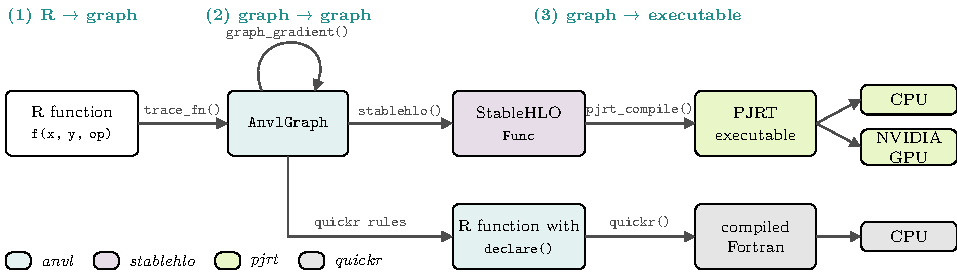
\includegraphics[width=\linewidth]{figures/overview.pdf}
\caption{The three kinds of transformations in \pkg{anvl}. A node's color indicates the package that implements it. Users call \code{jit()}, \code{gradient()}, and \code{value\_and\_gradient()}, which apply these steps once the types of the inputs are known.}
\label{fig:overview}
\end{figure}

\subsection{Arrays and eager execution}\label{eager}

The main data structure is the \code{AnvlArray}, which, compared to an \proglang{R} array, supports more data types, lives on a specific device, such as a CPU or a GPU, and represents scalars as arrays without axes.
Operations are available through \code{nv_*()} functions and the corresponding \proglang{R} generics, and called on arrays, they are executed immediately, which is called \emph{eager} execution.
An \code{AnvlArray} holds a buffer in device memory, which an \proglang{R} package would usually represent as an external pointer.
External pointers do not survive serialization, so objects holding them become invalid when they are saved with \code{saveRDS()} or sent to another \proglang{R} process, a common obstacle for \proglang{R} packages that manage foreign memory.
\pkg{pjrt} therefore wraps buffers in ALTREP objects \citep{ref-altrep}, whose serialization methods copy the data to the host and upload it again when the object is loaded, onto the default device of the loading session.
Arrays can thus be saved like any other \proglang{R} object and passed to parallel workers, e.g., via \pkg{parallel}, without explicit conversion.
Plain \proglang{R} values take the data type of the array they meet, so the literal \code{2} below becomes an \code{f32} (Section~\ref{precision}).

\begin{CodeChunk}
\begin{CodeInput}
R> library(anvl)
R> x <- nv_array(1:6, shape = c(2, 3), dtype = "f32")
R> sum(x * 2)
\end{CodeInput}
\begin{CodeOutput}
AnvlArray
 42
[ CPUf32{} ]
\end{CodeOutput}
\end{CodeChunk}

Under the hood, there are two layers of functions: \emph{primitives}, named \code{prim_*()}, are the minimal operations that the transformations know about, each defined by a set of rules, and the user-facing \code{nv_*()} functions build on them and add broadcasting of scalars, type promotion, and default arguments.
Each primitive is itself a jitted function, so eager execution compiles and caches one small program per primitive and input type; this is convenient for interactive work, but for performance, the whole program should be compiled.
Execution is asynchronous: calling a compiled program returns as soon as the computation has been scheduled, and its result is only awaited when its values are needed, e.g., by \code{as_array()}, which allows \proglang{R} to prepare the next call while the device is busy.
This matters because \proglang{R} itself is single-threaded and comparatively slow to dispatch work.
On a GPU, synchronous calls would leave the device idle while \proglang{R} prepares the next call, whereas with asynchronous execution, \proglang{R} enqueues work ahead of the device and the time spent in \proglang{R} is hidden, as long as each call does enough work.
On the CPU, the computation runs on XLA's own thread pool, so \proglang{R} can schedule programs on several devices from a single thread, which then run in parallel; the multi-chain benchmark in Section~\ref{runtime} uses this to run groups of chains on separate CPU devices.
Synchronization only happens where \proglang{R} needs the values, e.g., in \code{as_array()} or \code{await()}, and the latter is also what benchmarks have to call to measure the computation rather than its dispatch.

\subsection[An R-like array interface]{An \proglang{R}-like array interface}\label{rapi}

Array libraries such as \pkg{NumPy}, and with it \pkg{JAX} and \pkg{PyTorch}, follow \proglang{Python}'s conventions: 0-based indexing, row-major memory layout, and broadcasting that aligns shapes from the last axis.
\pkg{anvl} instead aims to feel familiar to \proglang{R} users, so that numerical code written for base \proglang{R} carries over with few changes.
Arrays have methods for about 100 \proglang{R} generics (Table~\ref{tab:overview}), whose semantics follow base \proglang{R}: indexing is 1-based, subsetting uses \proglang{R}'s bracket syntax, and arrays are laid out in column-major order, which matters whenever an operation traverses the elements of an array.
For example, \code{cumsum()} runs over a matrix column by column in both base \proglang{R} and \pkg{anvl}, whereas the same computation in \pkg{torch}, which requires flattening the tensor first, follows row-major order:

\begin{CodeChunk}
\begin{CodeInput}
R> m <- matrix(1:6, nrow = 2)
R> cumsum(m)
\end{CodeInput}
\begin{CodeOutput}
[1]  1  3  6 10 15 21
\end{CodeOutput}
\begin{CodeInput}
R> as_array(cumsum(nv_array(m)))
\end{CodeInput}
\begin{CodeOutput}
[1]  1  3  6 10 15 21
\end{CodeOutput}
\begin{CodeInput}
R> t <- torch::torch_flatten(torch::torch_tensor(m))
R> torch::as_array(torch::torch_cumsum(t, dim = 1))
\end{CodeInput}
\begin{CodeOutput}
[1]  1  4  9 11 15 21
\end{CodeOutput}
\end{CodeChunk}

Appendix~\ref{appendix-api} lists further operations of base \proglang{R}'s array interface that are hard to express or give surprising results, and how \pkg{anvl} handles them.
Where \pkg{anvl} needs functions of its own, their names and arguments follow base \proglang{R}, e.g., \code{nv_pmax()}, \code{nv_which_max()}, \code{nv_ifelse(test, yes, no)}, \code{nv_seq(from, to, by)}, and \code{nv_rnorm(shape, state, mean, sd)}.
\proglang{R} has no scalars, and its arrays cannot have zero axes: a number is a vector of length one, \code{array(1, dim = integer(0))} is an error, and a vector, which has no \code{dim}, is a different object from an array with one axis.
Whether a value is a scalar, a vector, or a matrix is therefore not part of its type, and code has to check it at run time, e.g., via \code{length(x) == 1}.
The missing distinction also explains why \proglang{R} needs a second subsetting operator for lists: as a single index is a vector of length one, \code{l[i]} cannot tell whether one element or a sublist of length one is requested and always returns a list, so the element itself has to be extracted with \code{l[[i]]}.
With scalar indices, as in \pkg{anvl}, where \code{x[i]} with a scalar index drops the axis and an array index keeps it, a single operator could express both.
In \pkg{anvl}, the shape of an array can have any length, including zero, so scalars, vectors, matrices, and arrays of higher rank are instances of one type whose number of axes is known: a reduction over all axes returns an array without axes, and the condition of \code{nv_if()} must be one.
This distinction matters in practice: in an analysis of a large corpus of \proglang{R} packages, \citet{ref-turcotte2020types} found that a third of all function arguments are scalars, and their proposed type language for \proglang{R} therefore distinguishes scalars from vectors.
One deliberate departure concerns how \proglang{R} values correspond to arrays.
A length-one \proglang{R} vector is a scalar, every other value must be an \proglang{R} array, whose \code{dim} becomes the shape, so each \proglang{R} value corresponds to exactly one shape.
The same principle applies to subsetting: in base \proglang{R}, \code{m[1, ]} drops an axis unless \code{drop = FALSE} is given, so the type of the result changes when the number of selected rows happens to be one.
In \pkg{anvl}, a scalar index drops the axis and an array index keeps it, whatever its length, which removes a discontinuity that would be particularly harmful in compiled programs, whose shapes are fixed:

\begin{CodeChunk}
\begin{CodeInput}
R> x <- nv_array(matrix(1:6, 2))
R> shape(x[1, ])
\end{CodeInput}
\begin{CodeOutput}
[1] 3
\end{CodeOutput}
\begin{CodeInput}
R> shape(x[array(1), ])
\end{CodeInput}
\begin{CodeOutput}
[1] 1 3
\end{CodeOutput}
\end{CodeChunk}

For broadcasting, \pkg{anvl} does not adopt \pkg{NumPy}'s general broadcasting rules, which align shapes from the last axis and silently turn, e.g., the sum of arrays of shape $(n)$ and $(n, 1)$ into an $n \times n$ matrix.
Base \proglang{R} has no broadcasting between arrays, but recycles vectors over the column-major elements of an array, which agrees with broadcasting only in some cases.
\pkg{anvl} therefore only broadcasts scalars automatically, as in \code{x * 2}, and general broadcasting is requested explicitly via \code{nv_broadcast_arrays()}, which aligns shapes from the first axis, the column-major counterpart of \pkg{NumPy}'s rule.
The remaining deviations from base \proglang{R} follow from static shapes and from functional purity.
Logical masks, as in \code{x[x > 6]}, work in eager execution, but inside \code{jit()} only if the mask is known during tracing, because the number of selected elements, and thus the shape of the result, depends on the values of the mask.
A mask computed from the inputs of a jitted function is therefore rejected, and the same result can usually be obtained by masking instead of selecting, e.g., \code{sum(nv_ifelse(x > 0, x, 0))} instead of \code{sum(x[x > 0])}.
Random number generators take and return an explicit state, because a compiled program cannot modify hidden global state such as \proglang{R}'s \code{.Random.seed}: a call to base \proglang{R}'s \code{rnorm()} inside a jitted function would be evaluated only once during tracing, and its values would be constants of the compiled program.

\subsection[Tracing R code into a graph]{Tracing \proglang{R} code into a graph}\label{trace}

Instead of statically analyzing the source code of a function, as \pkg{quickr} does, \pkg{anvl} \emph{traces} it: \code{trace_fn()} evaluates an \proglang{R} function with \code{GraphBox} objects in place of arrays, which carry only a data type and a shape.
Below, we trace a function that adds or multiplies two \code{f32} scalars, created by \code{nv_aval()}, depending on an argument \code{op}.

\begin{CodeChunk}
\begin{CodeInput}
R> f <- function(x, y, op) {
+    if (op == "add") x + y else x * y
+  }
R> s <- nv_aval("f32", integer())
R> graph <- trace_fn(f, list(x = s, y = s, op = "mul"))
R> graph
\end{CodeInput}
\begin{CodeOutput}
<AnvlGraph> (%x1: f32[], %x2: f32[]) {
  %1: f32[] = mul(%x1, %x2)
  return %1
}
\end{CodeOutput}
\end{CodeChunk}

Every call to a primitive appends a \code{GraphStatement}, consisting of the primitive, its inputs, its static parameters, and its outputs, to the graph, while all other \proglang{R} code is simply evaluated; here, only the branch of the \code{if} statement that was taken becomes part of the \code{AnvlGraph}.
Inputs and outputs are \emph{RTrees}, an \proglang{R} analog of \pkg{JAX}'s pytrees \citep{ref-jax}: arbitrarily nested lists, whose leaves are arrays or \proglang{R} values.
Before tracing, a tree is flattened into its leaves and its nesting structure is stored separately, and after execution, the outputs are restored into their tree, so transformed functions can take and return, e.g., a named list of model parameters, and \code{gradient()} returns the gradient in the same structure.

Compared to static analysis, tracing allows arbitrary \proglang{R} code to construct a program and only needs to know the semantics of the array operations, not those of the \proglang{R} language as a whole.
The downside is that tracing only works for functions that can be intercepted: \code{sum()} is a generic with a method for \pkg{anvl}'s arrays, whereas \code{rowSums()} is not generic and cannot be traced.
Furthermore, programs must be pure: side effects, such as printing, only happen once during tracing, and \proglang{R} control flow can only depend on values that are known during tracing, such as static arguments and shapes.

\subsection{Automatic differentiation}\label{ad}

AD computes derivatives of a program by applying the chain rule to the elementary operations it executes, whose derivatives are known \citep{ref-griewank2008evaluating}.
\emph{Forward mode} propagates derivatives from the inputs to the outputs alongside the evaluation, computing a Jacobian-vector product per pass, and is efficient for functions with few inputs.
\emph{Reverse mode} propagates the derivatives of the outputs with respect to each intermediate value, the \emph{adjoints}, backwards to the inputs, computing a vector-Jacobian product per pass, and thus yields the gradient of a scalar function with many parameters, such as a log-likelihood, at a small constant multiple of the cost of evaluating it.
Combining both, e.g., forward over reverse, gives Hessian-vector products and full Hessians efficiently.
\pkg{anvl} currently implements reverse mode.

\subsection{Transforming and lowering graphs}\label{lowering}

Once a program is represented as an \code{AnvlGraph}, it can be transformed into another graph.
Currently, the main such transformation is reverse-mode AD, e.g., \code{graph_gradient(graph, wrt = c("x", "y"))}.
For this, every primitive stores a \code{"reverse"} rule, which receives the inputs and outputs of the forward call and the adjoints of the outputs, and returns the vector-Jacobian products for the inputs.
\code{graph_gradient()} walks the graph in reverse order, applies these rules, and accumulates the adjoints of values that are used multiple times.
Because the reverse rules themselves call primitives, the backward pass is recorded with the same tracing machinery, and the result is again an \code{AnvlGraph}.

A backend then lowers a graph into an executable.
For the \code{"pjrt"} backend, \code{stablehlo()} translates the graph into a StableHLO function by applying each primitive's \code{"stablehlo"} rule, which maps it to one or more \pkg{stablehlo} operations and converts \proglang{R}'s 1-based indices to StableHLO's 0-based ones.
\proglang{R} literals are embedded into the program as constants, while arrays that the traced function closes over become additional inputs, which avoids copying their data into the program.
The result is compiled via \pkg{pjrt}.
The \pkg{quickr} backend instead translates the graph into an \proglang{R} function with type declarations and compiles it with \pkg{quickr}; compared to XLA, a compiled \pkg{quickr} function can be reused for inputs of different shapes, but it only runs on the CPU and supports fewer data types.

\subsection{The user interface}\label{ui}

Users rarely call these transformations themselves, but use \code{jit()}, \code{gradient()}, and \code{value_and_gradient()}, which return functions that apply them lazily, once the types of the inputs are known.
\code{jit()} returns a function that traces, lowers, and compiles its input when it is called, and caches the executable, so that a later call with inputs of the same data types and shapes reuses it.
Below, the side effect shows that the second call does not trace the function again.

\begin{CodeChunk}
\begin{CodeInput}
R> f_jit <- jit(function(x, y) {
+    cat("tracing\n")
+    x * y
+  })
R> y1 <- f_jit(x, x)
\end{CodeInput}
\begin{CodeOutput}
tracing
\end{CodeOutput}
\begin{CodeInput}
R> y2 <- f_jit(x, x + 1L)
\end{CodeInput}
\end{CodeChunk}

Arguments that are not arrays, such as \code{op} above, must be marked as \code{static}, e.g., \code{jit(f, static = "op")}; their values become part of the cache key, and the function is traced again for every new value.
A jitted function called from within another jitted function is traced as part of the outer function, so that both are compiled into a single executable.
\code{gradient()} takes a function with scalar output and returns a function that computes the gradient with respect to the arguments given in \code{wrt}, which can itself be called within a jitted function (Section~\ref{hmc}).

\proglang{R}'s control flow can be used within jitted functions, but an \code{if} statement only retains the branch that was taken and a loop is unrolled during tracing.
For control flow that depends on array values, or for loops that should not be unrolled, \pkg{anvl} provides the higher-order primitives \code{nv_if()}, \code{nv_while()}, and \code{nv_scan()}, which trace the functions passed to them into sub-graphs.
For example, \code{nv_scan()} runs a loop for a fixed number of steps, threads a state through a body function, and stacks the outputs of all steps; we use it in Section~\ref{hmc}.

The main restriction stems from XLA's requirement that all shapes are known when a program is compiled: each new combination of input shapes triggers a new compilation, and operations whose output shape depends on data, such as \code{unique()}, cannot be expressed directly (Section~\ref{limitations}).
Moreover, StableHLO programs cannot raise errors at runtime, so \pkg{anvl} performs all checks during tracing.

\subsection{Device memory}\label{memory}

\proglang{R} reclaims memory with a generational mark-and-sweep garbage collector, which runs when \proglang{R}'s own heap fills up; objects carry reference counts, but these only decide whether an object can be modified in place, and memory is reclaimed by the collector alone.
In contrast to \proglang{Python}, whose reference counting frees an object as soon as its last reference disappears, an object that goes out of scope in \proglang{R} is only freed the next time the collector runs.
An array on a GPU is represented in \proglang{R} by a small object that refers to device memory, so a loop that creates many such arrays barely grows \proglang{R}'s heap, the collector does not run, and device memory fills up with arrays that are no longer referenced.
This memory is only released by a collection, which marks all reachable \proglang{R} objects and blocks \proglang{R} in the meantime, so computations on the GPU end up waiting for \proglang{R}'s collector.
Packages that manage device memory from \proglang{R} therefore need a strategy of their own.
\pkg{torch} combines \pkg{PyTorch}'s caching allocator with a hook that runs \proglang{R}'s collector when an allocation fails or the reserved memory exceeds a threshold \citep{ref-torch-memory}.
\pkg{tensorflow} and \pkg{greta} rely on \proglang{Python}'s reference counting, which can only free a tensor once \proglang{R}'s collector has released its reference, and \pkg{TensorFlow} reserves most of the GPU memory for its own allocator by default.
\proglang{Stan} allocates \proglang{OpenCL} buffers within its \proglang{C++} code and frees them deterministically, so no device memory is visible to \proglang{R}.
For \pkg{anvl}, this is much less of a problem than for packages that execute every operation eagerly, such as \pkg{torch}, in which every intermediate result is an \proglang{R} object that holds on to its device memory until the collector runs.
In a jitted function, intermediate results never become \proglang{R} objects, but are buffers that XLA allocates, reuses, and frees, and inputs can be donated via the \code{donate} option of \code{jit()}, so that their memory is reused for the outputs.
Only the inputs and outputs of compiled programs and the results of eager operations are \proglang{R} objects, and when an allocation fails, \pkg{pjrt} runs \proglang{R}'s collector and retries, similar to \pkg{torch}.
On the CPU, arrays, including the results of compiled programs, are stored in memory allocated by \proglang{R}, so its collector accounts for them and runs when they fill up its heap.

\subsection{Data types and precision}\label{precision}

Numerical precision is a recurring concern in statistics: log-likelihoods sum many terms, linear systems can be ill-conditioned, and MCMC methods compare densities whose difference is small relative to their size.
Accelerators, on the other hand, are designed for single precision, and consumer GPUs often execute double-precision operations at a small fraction of the single-precision throughput.
A framework for statistical computing should therefore make it easy to choose the precision of a computation, and it should not lose precision without being asked to.

\subsubsection[R values have no data type]{\proglang{R} values have no data type}

In \pkg{JAX}, \proglang{Python} scalars are \emph{weakly typed}: they take the data type of the array they are combined with \citep{ref-jax}.
\pkg{NumPy} arrays, however, have a data type, and by default, \pkg{JAX} truncates double-precision data to single precision when it enters a program, while with 64-bit mode enabled, the data promotes every single-precision array it meets.
Transferred to \proglang{R}, where every real-valued vector is stored in double precision, either all data loses precision when it enters a program, or it pulls every computation into double precision.

\pkg{anvl} therefore extends weak typing to all \proglang{R} values that enter a program, i.e., length-one vectors as well as matrices and arrays.
An \proglang{R} value has no data type and only \emph{materializes} as an array when it meets one, taking its data type.
Below, the same \proglang{R} matrix \code{B} is multiplied with a single- and a double-precision array.

\begin{CodeChunk}
\begin{CodeInput}
R> B <- matrix(c(0.1, 0.2, 0.3, 0.4), 2, 2)
R> matmul <- jit(function(x, b) x %*% b)
R> c(dtype(matmul(nv_array(diag(2), dtype = "f32"), B)),
+    dtype(matmul(nv_array(diag(2), dtype = "f64"), B)))
\end{CodeInput}
\begin{CodeOutput}
[1] "f32" "f64"
\end{CodeOutput}
\end{CodeChunk}

In the second call, \code{B} enters the program in double precision and the product is exactly \code{B}, whereas a fixed default precision would either have lost precision or turned the first result into \code{f64}.
Only a value that meets no array, such as the argument of \code{nv_exp(1)}, settles on a default data type.
A non-static \proglang{R} argument of a jitted function, such as \code{b} above, enters the trace with a shape but no data type, and each operation that uses it decides at which data type it materializes; if it is used at several data types, it is transferred at the narrowest one that holds all of them.

The same principle guards against silent changes of values elsewhere.
An \proglang{R} value is built directly at the data type it takes, so a value that the data type cannot represent is an error: adding \code{-2L} to an unsigned 8-bit integer fails instead of wrapping around.
As in \proglang{R}, \code{x - 1L} keeps an integer array \code{x} an integer, while \code{x - 1} gives a float.
Finally, integers never become floats on their own: an unsigned and a signed 64-bit integer have no common data type and must be converted explicitly, whereas \pkg{JAX} and \pkg{NumPy} silently promote them to a float.

\subsubsection{Choosing the precision}

The default data types for \proglang{R} doubles and integers are a property of the backend (\code{f32} and \code{i32} for XLA) and can be changed for a scope via \code{with_default_dtypes()} or the option \code{anvl.default_dtypes}.
\code{with_dtypes()} turns a function into one that runs at the given data types, converting its array arguments and results and setting the defaults for its body.

\begin{CodeChunk}
\fitcode
\begin{CodeInput}
R> loss <- function(beta, X, y) mean((X %*% beta - y)^2)
R> loss_f64 <- with_dtypes(loss, c(float = "f64"))
R> c(dtype(nv_exp(1)), dtype(with_default_dtypes(c(float = "f64"), nv_exp(1))),
+    dtype(loss_f64(nv_array(matrix(0, 2, 2), dtype = "f32"), B, B)))
\end{CodeInput}
\begin{CodeOutput}
[1] "f32" "f64" "f64"
\end{CodeOutput}
\end{CodeChunk}

Compiled programs are cached per default data types, so both variants can be used side by side, and in contrast to \pkg{JAX}'s 64-bit mode, the defaults only decide what an \proglang{R} value settles on when nothing else determines its data type.

\subsubsection{Promotion rules}

When a function receives arrays of different data types, it has to decide on the data type of the computation.
In \pkg{anvl}, this is not a global rule, but each \code{nv_*()} function passes a \emph{promotion rule} to \code{as_anvl_arrays()}, which converts its arguments to arrays at the beginning of the function.
\code{promotion_common()} brings all inputs to their common data type, as used, e.g., by \code{nv_add()}; \code{promotion_like()} brings them to the data type of one designated input; \code{promotion_dtype()} to a fixed data type; and \code{promotion_rdata_common()}, which is used by primitives, only lets \proglang{R} values adapt and requires arrays to agree.
The rules refuse conversions that lose precision unless \code{coerce = TRUE}.
For example, the following function computes $a x + y$ at the data type of \code{y}, and refuses an \code{x} of higher precision rather than silently rounding it.

\begin{CodeChunk}
\fitcode
\begin{CodeInput}
R> axpy <- jit(function(a, x, y) {
+    args <- as_anvl_arrays(a = a, x = x, y = y, .promote = promotion_like("y"))
+    args$a * args$x + args$y
+  })
R> y32 <- nv_array(c(1, 1), dtype = "f32")
R> as_array(axpy(2, nv_array(c(1, 2), dtype = "f32"), y32))
\end{CodeInput}
\begin{CodeOutput}
[1] 3 5
\end{CodeOutput}
\begin{CodeInput}
R> axpy(2, nv_array(c(1, 2), dtype = "f64"), y32)
\end{CodeInput}
\begin{CodeOutput}
Error:
! Cannot bring `x` to data type "f32".
x "f64" is not promotable to "f32".
i Convert it explicitly with `nv_convert()`.
\end{CodeOutput}
\end{CodeChunk}

Developers of packages built on \pkg{anvl} can thus decide for each function which argument determines the precision, e.g., that a likelihood is accumulated in double precision while the data stays in single precision.

\subsection{Other features}\label{features}

Beyond the transformations, \pkg{anvl} provides several practical features, some of which are described in more detail above.
\begin{itemize}
\item \emph{No CUDA toolkit}: \code{install_anvl()} downloads the PJRT plugins and, on a machine with an NVIDIA GPU, installs the CUDA libraries as the \proglang{R} package \pkg{pjrt.cuda}, so a compatible NVIDIA driver is all that is needed.
\item \emph{Serializable arrays}: arrays can be saved with \code{saveRDS()} and passed to parallel workers like any other \proglang{R} object (Section~\ref{eager}), and \code{nv_save()} and \code{nv_read()} write and read files in the safetensors format.
\item \emph{All CPU cores}: XLA parallelizes operations over all cores of the CPU without any configuration (Section~\ref{runtime}).
\item \emph{Asynchronous execution}: \proglang{R} continues while the device computes (Section~\ref{eager}).
\item \emph{Nested lists of arrays}: jitted functions and gradients take and return nested lists of arrays, such as a named list of model parameters (Section~\ref{trace}).
\item \emph{An alternative backend}: the experimental \pkg{quickr} backend translates programs to \proglang{Fortran} (Section~\ref{lowering}).
\item \emph{Written in \proglang{R}}: except for the PJRT runtime, \pkg{anvl} and \pkg{stablehlo} are written in \proglang{R}, which makes them easy to read, extend, and contribute to (Section~\ref{extending}).
\item \emph{Error messages}: errors say what went wrong and how to fix it, as in the promotion example in Section~\ref{precision}.
\end{itemize}

\section{Extending the package}\label{extending}

Most operations can be expressed in terms of existing primitives and are best added as \code{nv_*()} functions.
A new primitive is needed if an operation cannot be expressed otherwise, or if it benefits from a dedicated implementation, e.g., of its derivative.
Below, we add a primitive for the softplus function $\log(1 + e^x)$, which appears in the logistic regression example in Section~\ref{hmc}.
A primitive is created via \code{new_primitive()}, whose body records a statement in the graph via \code{graph_desc_add()}, together with an inference function that computes the types of the outputs from those of the inputs and validates them.
Within the body, \code{self} refers to the primitive being defined.

\begin{CodeChunk}
\begin{CodeInput}
R> prim_softplus <- new_primitive("softplus", function(x) {
+    infer <- function(x) {
+      if (!(dtype(x) %in% c("f32", "f64"))) stop("`x` must be a float.")
+      list(AbstractArray(dtype = dtype(x), shape = shape(x)))
+    }
+    graph_desc_add(self, list(x = x), infer_fn = infer)[[1L]]
+  })
\end{CodeInput}
\end{CodeChunk}

Next, we attach the StableHLO rule, which receives and returns \pkg{stablehlo} values, and a reverse rule, which uses the derivative $\sigma(x) = 1 / (1 + e^{-x})$.

\begin{CodeChunk}
\begin{CodeInput}
R> prim_softplus[["stablehlo"]] <- function(x) {
+    list(hlo_log_plus_one(hlo_exponential(x)))
+  }
R> prim_softplus[["reverse"]] <- rule_reverse(
+    function(inputs, outputs, grads, params, required) {
+      list(prim_mul(grads[[1L]], prim_plogis(inputs[[1L]])))
+    }
+  )
\end{CodeInput}
\end{CodeChunk}

The primitive can now be used eagerly, within jitted functions, and be differentiated.

\begin{CodeChunk}
\begin{CodeInput}
R> grad_softplus <- jit(gradient(function(z) sum(prim_softplus(z))))
R> as_array(grad_softplus(nv_array(c(-1, 0, 1)))$z)
\end{CodeInput}
\begin{CodeOutput}
[1] 0.2689414 0.5000000 0.7310586
\end{CodeOutput}
\end{CodeChunk}

Operations that cannot be expressed in StableHLO can use PJRT's custom call mechanism: a handler written in \proglang{C} or \proglang{C++} against XLA's foreign function interface is registered from \proglang{R} via \pkg{pjrt}, with separate implementations per platform, as the linear algebra primitives do to call LAPACK and cuSOLVER.

Since an \code{AnvlGraph} is a simple data structure, new graph-to-graph transformations, such as forward-mode AD, can be implemented in \proglang{R} by iterating over its statements and emitting new ones, guided by a rule stored in each primitive.
A backend is an \code{AnvlBackend} object, a collection of functions that define how arrays are stored, converted to \proglang{R}, and placed on devices, and how a graph is compiled, together with a lowering rule for each supported primitive; exactly one backend is active at a time.
We test every primitive against \pkg{torch} as a reference implementation wherever possible, comparing the outputs and gradients of jitted primitives with those of \pkg{torch} and its autograd engine on random inputs.

\section{Use case: Hamiltonian Monte Carlo}\label{hmc}

Hamiltonian Monte Carlo (HMC) \citep{ref-neal2011mcmc} is an MCMC method that uses the gradient of the log posterior density to propose distant states that are still accepted with high probability, and thus a natural use case for \pkg{anvl}: it needs gradients, its loops are slow in \proglang{R}, and running many chains in parallel is a good fit for GPUs.
We consider Bayesian logistic regression with a binary response $y \in \{0, 1\}^n$, features $X \in \R^{n \times p}$, $y_i \sim \text{Bernoulli}(\sigma(x_i^\top \beta))$, and a standard normal prior $\beta \sim \mathcal{N}(0, I_p)$.
HMC simulates the dynamics of a particle with position $\beta$ and momentum $\rho \sim \mathcal{N}(0, I_p)$ in the potential energy
\[U(\beta) = -\log p(\beta \mid X, y) = -\sum_{i = 1}^n \left(y_i x_i^\top \beta - \log(1 + e^{x_i^\top \beta})\right) + \frac{1}{2}\lVert \beta \rVert^2 + \text{const}.\]
We write the sampler for $K$ chains at once, so the positions are stored in a $K \times p$ matrix, and the potential returns a vector of length $K$.

\begin{CodeChunk}
\begin{CodeInput}
R> potential <- function(beta, X, y) {
+    eta <- X %*% t(beta)
+    y <- nv_broadcast_to(y, shape(eta))
+    loglik <- nv_sum(y * eta - nv_log1p(exp(eta)), axes = 1L)
+    logprior <- -nv_sum(beta^2, axes = 2L) / 2
+    -(loglik + logprior)
+  }
\end{CodeInput}
\end{CodeChunk}

Because the chains are independent, the gradient of the summed potential contains the gradient of each chain in the corresponding row, so a single call to \code{gradient()} yields the gradients of all chains.

\begin{CodeChunk}
\begin{CodeInput}
R> grad_potential <- gradient(
+    function(beta, X, y) sum(potential(beta, X, y)),
+    wrt = "beta"
+  )
\end{CodeInput}
\end{CodeChunk}

The dynamics are simulated with the leapfrog integrator, which alternates half steps of size $\varepsilon/2$ for the momentum with full steps of size $\varepsilon$ for the position.
We run $L$ such steps with \code{nv_scan()}, where the gradient at the current position is part of the carry, so that each step evaluates the gradient only once.

\begin{CodeChunk}
\begin{CodeInput}
R> leapfrog <- function(beta, p, X, y, eps, L) {
+    init <- list(beta = beta, p = p, grad = grad_potential(beta, X, y)$beta)
+    nv_scan(init, steps = L, body = function(s, x) {
+      p <- s$p - eps / 2 * s$grad
+      beta <- s$beta + eps * p
+      grad <- grad_potential(beta, X, y)$beta
+      p <- p - eps / 2 * grad
+      list(carry = list(beta = beta, p = p, grad = grad), out = NULL)
+    })$carry
+  }
\end{CodeInput}
\end{CodeChunk}

A transition draws a new momentum, simulates a trajectory, and accepts the proposal of each chain with probability $\min(1, \exp(H_0 - H_1))$, where $H = U(\beta) + \lVert \rho \rVert^2 / 2$ is the total energy.
The random number generator state is passed explicitly, and the acceptance decision uses \code{nv_ifelse()} instead of an \proglang{R} \code{if} statement, as it depends on array values.

\begin{CodeChunk}
\begin{CodeInput}
R> hmc_step <- function(beta, state, X, y, eps, L) {
+    draw <- nv_rnorm(shape(beta), state)
+    p <- draw$values
+    prop <- leapfrog(beta, p, X, y, eps, L)
+    H0 <- potential(beta, X, y) + nv_sum(p^2, axes = 2L) / 2
+    H1 <- potential(prop$beta, X, y) + nv_sum(prop$p^2, axes = 2L) / 2
+    u <- nv_runif(shape(beta)[1L], draw$state)
+    accept <- log(u$values) < H0 - H1
+    accept <- nv_broadcast_to(accept, shape(beta))
+    list(beta = nv_ifelse(accept, prop$beta, beta), state = u$state)
+  }
\end{CodeInput}
\end{CodeChunk}

Finally, we collect \code{n_draws} draws with another \code{nv_scan()}, whose outputs are stacked along a new first axis, and compile the whole sampler with \code{jit()}.
The number of leapfrog steps and draws are static arguments, as they determine the structure of the program.

\begin{CodeChunk}
\begin{CodeInput}
R> hmc <- jit(function(beta, state, X, y, eps, L, n_draws) {
+    out <- nv_scan(list(beta = beta, state = state), steps = n_draws,
+      body = function(s, x) {
+        s <- hmc_step(s$beta, s$state, X, y, eps, L)
+        list(carry = s, out = s$beta)
+      }
+    )
+    list(draws = out$out, beta = out$carry$beta, state = out$carry$state)
+  }, static = c("L", "n_draws"))
\end{CodeInput}
\end{CodeChunk}

We apply the sampler to simulated data with $n = 1000$ observations and $p = 5$ features, running four chains in double precision.
The posterior means, computed from the second half of each chain, agree with the maximum likelihood estimates up to the shrinkage induced by the prior.

\begin{CodeChunk}
\begin{CodeInput}
R> options(anvl.default_dtypes = c(float = "f64", int = "i32"))
R> set.seed(1)
R> n <- 1000; p <- 5
R> X <- matrix(rnorm(n * p), n, p)
R> y <- rbinom(n, 1, plogis(X %*% rnorm(p, sd = 0.5)))
R> res <- hmc(nv_array(matrix(0, 4, p)), nv_rng_state(42L), nv_array(X),
+    nv_array(as.double(y)), eps = 0.5 / sqrt(n), L = 10L, n_draws = 2000L)
R> draws <- as_array(res$draws)
R> rbind(hmc = colMeans(apply(draws[1001:2000, , ], 3, c)),
+    glm = coef(glm(y ~ X - 1, family = binomial)))
\end{CodeInput}
\begin{CodeOutput}
            X1        X2         X3        X4        X5
hmc -0.7730560 0.3412134 -0.8296505 0.6687511 0.5593170
glm -0.7738017 0.3425455 -0.8321399 0.6701697 0.5599573
\end{CodeOutput}
\end{CodeChunk}

The whole sampler, including the $2000 \times 11$ gradient evaluations per chain, runs as a single compiled program without returning to \proglang{R}.
The same code runs on a GPU when the arrays are allocated there, e.g., via \code{nv_array(X, device = "cuda")}.

\section{Runtime evaluation}\label{runtime}

We compare the runtime of the HMC sampler from Section~\ref{hmc} to \proglang{Stan}, whose AD library and code generation are the state of the art for statistical models on the CPU \citep{ref-stanmath}, to \pkg{TMB}, and to the same sampler written with \pkg{torch}.

\subsection{Setup}

We run \proglang{Stan}'s static HMC sampler (without the No-U-Turn extension) via CmdStan 2.40 with the same step size $\varepsilon = 0.5/\sqrt{n}$, $L = 10$ leapfrog steps, the identity metric, and adaptation disabled, so that all samplers perform the same number of gradient evaluations.
The \proglang{Stan} model uses \code{bernoulli_logit_glm()}, \proglang{Stan}'s most efficient implementation of the logistic regression likelihood, which can also be evaluated on a GPU via \proglang{OpenCL}; on the GPU, \proglang{Stan}'s chains run as separate processes that share the device, at most 8 at a time.
\pkg{TMB} evaluates the log posterior and its gradient with \pkg{CppAD} from a \proglang{C++} template, and as it does not provide an HMC sampler, we run the same static HMC loop in \proglang{R} around its compiled objective and gradient, as is common when custom algorithms are implemented with \pkg{TMB}.
The \pkg{torch} sampler mirrors the \pkg{anvl} code, but runs the leapfrog and sampling loops in \proglang{R}, as \pkg{torch} executes each operation eagerly.
All samplers work in double precision and start at $\beta = 0$, and the data are simulated with standard normal features and $\beta \sim \mathcal{N}(0, 0.25 I_p)$.
We exclude process start-up and data loading from \proglang{Stan}'s measurements by subtracting the time of an otherwise identical run without draws, and time \pkg{anvl} after the data has been transferred to the device.
Each configuration is repeated three times after a first call that includes compilation, and we report the median.

We run three experiments.
First, we draw 1000 samples from a single chain for $p = 20$ and $n \in \{10^3, 10^4, 10^5\}$.
Second, we measure strong scaling: we draw 200 samples from a single chain for $n = 10^5$ and $p = 100$ on 1 to 16 cores.
\pkg{anvl} and \pkg{torch} run the unchanged sampler, which they parallelize within operations, \pkg{TMB} evaluates the likelihood with several OpenMP threads, and \proglang{Stan} needs a modified model, in which \code{reduce_sum()} splits the likelihood into slices that are evaluated by several threads.
Third, we draw 1000 samples from each of $K$ chains for $n = 10^4$ and $p = 20$.
CmdStan and \pkg{TMB} run one chain per process, at most one per core, and \pkg{anvl} runs all chains as one batched program, except on 16 cores, where we split them into 16 groups that run on separate PJRT CPU devices.
All experiments ran on the LRZ AI Systems, on two Intel Xeon Gold 6336Y processors restricted to 16 physical cores and on an NVIDIA A100 80GB GPU, in a \pkg{Docker} image that pins all software versions; the image, the benchmark scripts, and instructions are in the \code{paper/} directory of \url{https://github.com/r-xla/anvl}.

\subsection{Results}

\begin{figure}[tbp]
\centering
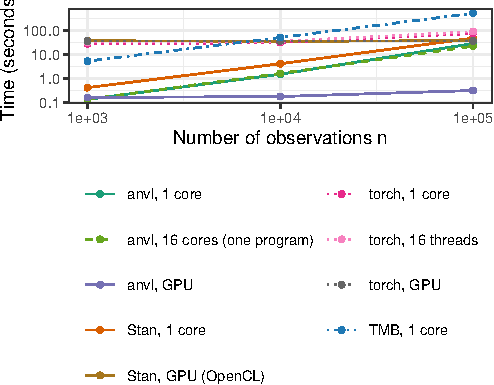
\includegraphics[width=0.48\linewidth]{figures/runtime-single-chain.pdf}
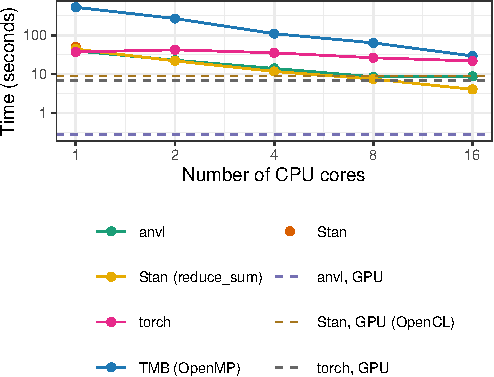
\includegraphics[width=0.48\linewidth]{figures/runtime-strong-scaling.pdf}
\caption{Left: time to draw 1000 samples from a single chain as a function of the number of observations $n$ ($p = 20$). Right: strong scaling, time to draw 200 samples from a single chain for $n = 10^5$ and $p = 100$ on 1 to 16 CPU cores; \proglang{Stan} uses \code{reduce\_sum()}, the single point is the unmodified \proglang{Stan} model, and the dashed lines are \pkg{anvl}, \pkg{torch}, and \proglang{Stan} (\proglang{OpenCL}) on the GPU. Medians of three repetitions, log-log scales.}
\label{fig:results-single-scaling}
\end{figure}

Figure~\ref{fig:results-single-scaling} (left) shows the results for a single chain.
On one core, \pkg{anvl} draws the samples 3.1, 2.7, and 1.7 times faster than CmdStan for $n = 10^3$, $10^4$, and $10^5$, respectively.
A plausible reason is that XLA compiles the whole sampler into a single optimized program, whereas \proglang{Stan} and \pkg{TMB}, which takes 11 to 13 times as long as CmdStan, evaluate the gradient with operator-overloading AD.
The GPU does not pay off for small data, but for $n = 10^5$, it draws the samples in 0.31 seconds, about 90 times faster than \pkg{anvl} on one core and 150 times faster than CmdStan.
The \pkg{torch} sampler needs about 28 seconds for $n = 10^3$ on one core, 200 times as long as \pkg{anvl}, and about 36 seconds for every $n$ on the GPU: its runtime is dominated by the overhead of dispatching each operation from \proglang{R}, which is the per-operation overhead of eager execution discussed in Section~\ref{in-r}.
\proglang{Stan}'s \proglang{OpenCL} backend, which evaluates only the likelihood and its gradient on the GPU, needs 35 to 38 seconds for every $n$, as each gradient evaluation transfers data and launches kernels.

Figure~\ref{fig:results-single-scaling} (right) shows how a single chain scales with the number of cores.
Without any change to the code, \pkg{anvl} becomes 1.7, 2.8, and 4.6 times faster on 2, 4, and 8 cores, and does not improve further on 16 cores, where the individual operations are too small at this problem size to keep all cores busy.
With \code{reduce_sum()}, \proglang{Stan} scales further (11 times faster on 16 threads), but this requires rewriting the model, which is then slower on a single core (44 versus 50 seconds, compared to 39 seconds for \pkg{anvl}).
\pkg{TMB} becomes 18 times faster on 16 threads, but starts from 522 seconds, and \pkg{torch} is as fast as \pkg{anvl} on one core, where the operations are large enough to hide its overhead, but becomes only 1.7 times faster on 16 threads.
% The three numbers below are inline R results in paper.Rmd (medians of the scaling-gpu*.csv results).
On the GPU, the same run takes 0.28 seconds with \pkg{anvl}, 7 seconds with \pkg{torch}, and 8.9 seconds with \proglang{Stan}'s \proglang{OpenCL} backend.

\begin{figure}[tbp]
\centering
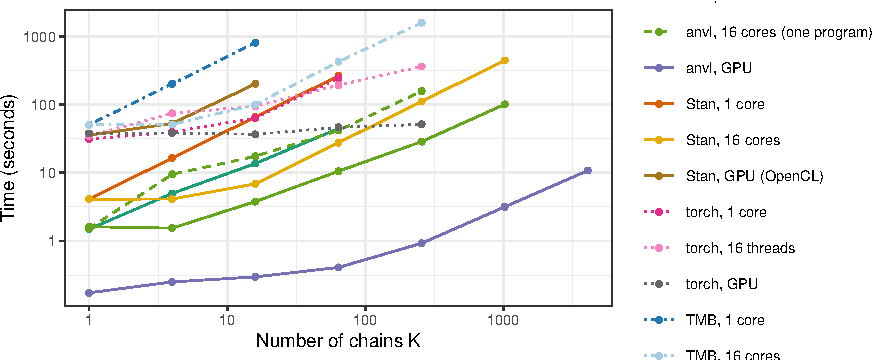
\includegraphics[width=\linewidth]{figures/runtime-multiple-chains.pdf}
\caption{Time to draw 1000 samples from each of $K$ chains for $n = 10^4$ (median of three repetitions, log-log scale).}
\label{fig:results-chains}
\end{figure}

Figure~\ref{fig:results-chains} shows the results for multiple chains.
On one core, \pkg{anvl} is 2.8 (one chain) to 5.9 (64 chains) times faster than CmdStan, as batching turns the matrix-vector products of the individual chains into matrix-matrix products.
\pkg{torch} benefits from batching as well, but is still 5.5 times slower than \pkg{anvl} for 64 chains on one core, and \pkg{TMB} takes 55 to 59 times as long as \pkg{anvl}.
On 16 cores, \pkg{anvl} is 2.6 times faster than CmdStan for 64 chains and 4.4 times faster for 1024 chains; running all chains as a single program instead of splitting them over devices is considerably slower, because each operation is again too small to be distributed efficiently.
On the GPU, the time of \pkg{anvl} is almost constant up to 64 chains and grows sublinearly beyond: 4096 chains with 1000 draws each take 10.8 seconds, about 380,000 draws per second, compared to 2,300 for CmdStan on 16 cores.
This is the regime in which the many-chain MCMC methods discussed in the introduction operate; on the GPU, \pkg{torch} did not finish 1024 chains and \proglang{Stan}'s \proglang{OpenCL} backend did not finish 64 chains within one hour.
All average acceptance rates were between 0.97 and 0.99.

Finally, the one-off costs are small: for $n = 10^4$ on 16 cores, tracing the sampler, lowering it to StableHLO, and compiling it with XLA take 0.28, 0.21, and 0.24 seconds, respectively, compared to about 11 seconds for compiling the \proglang{Stan} model and 35 seconds for the \pkg{TMB} template.

\section{Limitations}\label{limitations}

Most limitations of \pkg{anvl} follow from XLA's requirement that all shapes are known when a program is compiled, and from the transformations that \pkg{anvl} does not implement yet.

\paragraph{Static shapes.}
Because XLA compiles a program for fixed shapes, \code{jit()} traces and compiles a function anew for every combination of input shapes it is called with (Section~\ref{ui}).
For the HMC sampler, tracing, lowering, and compilation together take about 0.7 seconds (Section~\ref{runtime}), which is negligible when a function is called many times with the same shapes, as in a sampler or an optimizer, but adds up when the shapes change from call to call, e.g., when the same model is fitted to many data sets of different sizes.
Operations whose output shape depends on the values of their inputs cannot be part of a compiled program at all: selecting elements with a logical mask that is computed inside the program, as in \code{x[x > 0]} (Section~\ref{rapi}), or \code{unique()}.
For the same reason, the state of \code{nv_while()} and \code{nv_scan()} keeps its shape across iterations, so an algorithm that collects a varying number of values has to preallocate an array of the maximal size.
Such programs can usually be rewritten: masking replaces selection, e.g., \code{sum(nv_ifelse(x > 0, x, 0))} instead of \code{sum(x[x > 0])}, padding inputs to a few fixed sizes bounds the number of compilations, and steps whose output shape depends on the data can run eagerly or in plain \proglang{R} between calls of jitted functions.
The \pkg{quickr} backend, whose compiled functions can be reused for inputs of different shapes (Section~\ref{lowering}), and the IREE compiler \citep{ref-iree}, which also consumes StableHLO and supports dynamic shapes, are two routes towards lifting this restriction.

\paragraph{Automatic differentiation.}
\pkg{anvl} implements only reverse mode (Section~\ref{ad}), and \code{gradient()} only differentiates functions with a scalar output.
Jacobians and Hessians therefore have to be assembled from one reverse pass per output, whereas \pkg{JAX} combines forward and reverse mode to compute them more efficiently.
Reverse mode differentiates through \code{nv_if()} and \code{nv_scan()}, but not through \code{nv_while()}: the number of iterations of a while loop is only known at runtime, so there is no static size for the intermediate values of all iterations, which the backward pass needs.
Loops with a fixed number of iterations should therefore be written with \code{nv_scan()}.

\paragraph{Vectorization and multiple devices.}
\pkg{anvl} has no vectorizing transformation like \pkg{JAX}'s \code{vmap()}, so batched code, such as the multi-chain sampler in Section~\ref{hmc}, has to be written by hand.
Each array resides on a single device, and a program runs on the device of its inputs.
Several devices can be used by running separate programs on them, as in the multi-chain benchmark in Section~\ref{runtime}, but a single program cannot be distributed over several devices, as \pkg{JAX} does by sharding arrays.

\paragraph{Hardware and data types.}
Although XLA also targets further accelerators, \pkg{anvl} currently supports only CPUs and NVIDIA GPUs, and the \pkg{quickr} backend is experimental, runs only on the CPU, and supports fewer data types.
Floating-point computations are supported in single and double precision (Table~\ref{tab:overview}); half-precision types, which are common in deep learning, and complex numbers are not supported.

\section{Conclusion}\label{discussion}

We introduced \pkg{anvl}, which brings composable code transformations for array programs to \proglang{R}: programs are traced into a graph, which can be differentiated in reverse mode and compiled via OpenXLA or \pkg{quickr}, so the same \proglang{R} code runs on CPUs and GPUs, with an \proglang{R}-like array interface and control over numerical precision.
The HMC use case showed that a whole sampler can be compiled into a single program that is faster than \proglang{Stan} on the CPU and scales to thousands of chains on a GPU.

Its main limitations are XLA's static shapes and the restriction of AD to reverse mode (Section~\ref{limitations}).
Future work will add forward-mode AD, which, combined with reverse mode, yields Jacobians and Hessians efficiently, e.g., for Laplace approximations, and a vectorizing transformation similar to \pkg{JAX}'s \code{vmap()}, which would remove the need to write batched code by hand.
Beyond the core, we hope that \pkg{anvl} will serve as a foundation for packages that implement statistical and machine learning algorithms, such as samplers and variational inference, on top of it.
A first such package is \pkg{garry} \citep{ref-garry}, a lazy raster engine for remote sensing that compiles the numerical kernels of a raster computation with \pkg{anvl} and executes them chunked across processes.

\section*{Acknowledgments}

Sebastian Fischer is supported by the Deutsche Forschungsgemeinschaft (DFG, German Research Foundation) under the National Research Data Infrastructure - NFDI 29/2 - project number 460135501
We thank the developers of \pkg{JAX}, whose design and documentation, in particular the Autodidax tutorial \citep{ref-autodidax}, inspired many aspects of \pkg{anvl}, as well as the authors of the \proglang{Go} library \pkg{gopjrt} \citep{ref-gopjrt}, which informed the design of \pkg{pjrt}.
The computations were run using resources provided by the Leibniz Supercomputing Centre (LRZ).

\bibliography{references}

\begin{appendix}

\section[Pitfalls of base R's array interface]{Pitfalls of base \proglang{R}'s array interface}\label{appendix-api}

Base \proglang{R}'s array interface grew around vectors, and several of its rules give results that depend on the length of an index or argument rather than on its meaning.
In interactive use, such results are noticed and corrected, but in a compiled program, whose shapes are fixed, they would become hard-to-find bugs or prevent compilation altogether.
Table~\ref{tab:pitfalls} lists the cases we encountered most often and how \pkg{anvl} handles them; the code for each case is part of the replication material.

\begin{table}[tbp]
\centering
\small
\begin{tabular}{@{}>{\raggedright\arraybackslash}p{0.22\textwidth}>{\raggedright\arraybackslash}p{0.36\textwidth}>{\raggedright\arraybackslash}p{0.36\textwidth}@{}}
\hline
Operation & Base \proglang{R} & \pkg{anvl} \\
\hline
\code{m[i, ]} with \code{length(i) == 1} & drops the axis unless \code{drop = FALSE} & a scalar index drops the axis, an array index keeps it, whatever its length \\
\code{x[-i]} with \code{i = integer(0)} & returns an empty vector instead of \code{x} & negative indices are not supported; masks select elements \\
\code{x + y} with different lengths & recycles the shorter vector, warning only if the lengths do not divide & an error; only scalars are broadcast \\
\code{m + r} for a $2 \times 3$ matrix \code{m} and a $1 \times 3$ matrix \code{r} & an error; requires \code{sweep()} & explicit broadcasting via \code{nv_broadcast_arrays()} \\
\code{cumsum()}, \code{sort()}, \code{rev()} of a matrix & flatten the matrix & operate along a given axis and keep the shape \\
reduction over the second axis of a 3-d array & requires \code{apply()}, which loops in \proglang{R} & \code{nv_sum(x, axes = 2)} for any set of axes \\
\code{A \%*\% B} for 3-d arrays \code{A}, \code{B} & silently returns the inner product of the flattened arrays & batched matrix product along the leading axes \\
\code{v \%*\% v} for a vector \code{v} & a $1 \times 1$ matrix; vectors silently become rows or columns & an error; operands need at least two axes \\
integer overflow, other data types & \code{NA} with a warning; no single precision, 64-bit, or unsigned integers & explicit data types; values that a data type cannot hold are an error \\
\code{sample(x)} with \code{length(x) == 1} & samples from \code{1:x} & \code{nv_sample()} always samples from the given array \\
\hline
\end{tabular}
\caption{Operations of base \proglang{R}'s array interface that are hard to express or give surprising results, and their counterparts in \pkg{anvl}.}
\label{tab:pitfalls}
\end{table}

\section{Missing values}\label{appendix-na}

\proglang{R} represents missing values by special values of its data types: \code{NA_real_} is a NaN with a particular payload, \code{NA_integer_} is the smallest 32-bit integer, and a logical \code{NA} has no counterpart in a boolean type.
Array libraries and compilers that are not specific to \proglang{R} do not know these conventions, so missing values can change their meaning when data enters or leaves a program.
Table~\ref{tab:missing-values} shows what the packages compared in Table~\ref{tab:comparison} return for \proglang{R}'s missing values after passing them through a minimal program, and whether \code{NA_integer_ + 1L} still yields \code{NA}, as in \proglang{R}.
The table is generated by the script \code{verification/missing_values.R} in the replication material.

% Rendered from verification/missing_values.csv (chunk missing-values in paper.Rmd).
\begin{table}[tbp]
\centering
\begin{tabular}{lllll}
\hline
Package & Double \code{NA} & Integer \code{NA} & \code{NA\_integer\_ + 1L} & Logical \code{NA} \\
\hline
\pkg{anvl} & kept & kept (warning) & -2147483647 & error \\
\pkg{torch} & kept & kept & -2147483647 & TRUE \\
\pkg{tensorflow} & kept & kept & -2147483647 & TRUE \\
\pkg{greta} & error & error & -- & error \\
\pkg{quickr} & kept & kept & -2147483647 & TRUE \\
\pkg{ast2ast} & kept & kept & NA & kept \\
\proglang{Stan} & error & error & -- & error \\
\pkg{TMB} & kept & 0 & -- & 0 \\
\pkg{RTMB} & kept & kept & -- & kept \\
\pkg{nimble} & kept & kept & -2147483647 & TRUE \\
\hline
\end{tabular}
\caption{Missing values after a round trip through a minimal program of each package. kept: \proglang{R} recognizes the result as missing again; error: the package refuses the value; otherwise the value the missing value turned into. The integer column of \pkg{RTMB} uses doubles, as its tapes only support doubles.}
\label{tab:missing-values}
\end{table}

For doubles, most packages return \code{NA} unchanged, as the NaN payload happens to survive the computation, while \pkg{greta} and \proglang{Stan} refuse missing values.
For integers, only \pkg{ast2ast} treats \code{NA_integer_} as missing in arithmetic; in the other packages, including \pkg{anvl}, it is an ordinary integer inside the program, and \code{NA_integer_ + 1L} silently yields $-2^{31} + 1$, of which \pkg{anvl} only warns when the value returns to \proglang{R}.
A logical \code{NA}, finally, silently becomes \code{TRUE} or 0 in most packages, whereas \pkg{anvl} refuses it.

\end{appendix}

\end{document}
